
\documentclass{report}
\usepackage[T1]{fontenc} % Fontes T1
\usepackage[utf8]{inputenc} % Input UTF8
\usepackage[nottoc]{tocbibind}
\usepackage{csquotes}
\usepackage[portuguese]{babel} %Usar língua portuguesa
\usepackage{blindtext} % Gerar texto automaticamentez	
\usepackage[printonlyused]{acronym}
\usepackage{hyperref} % para autoref
\usepackage{graphicx}



\begin{document}
%%
% Definições
%

\def\titulo{Trabalho de aprofundamento AP2}
\def\data{9 de Abril de 2019}
\def\autores{André Patacas, Gil Teixeira}
\def\autorescontactos{(93357) andrepatacas@ua.pt, (88194) gilteixeira@ua.pt}
\def\departamento{DETI}
\def\logotipo{ua.pdf}
%
%%%%%% CAPA %%%%%%
%
\begin{titlepage}

\begin{center}
%
\vspace*{50mm}
%
{\Huge \titulo}\\ 
%
\vspace{10mm}
%
{\LARGE \autores}\\ 
%
\vspace{30mm}
%
\begin{figure}[h]
\center
\includegraphics{\logotipo}
\end{figure}
%
\vspace{30mm}
\end{center}
%
\begin{flushright}

\end{flushright}
\end{titlepage}

%%  Página de Título %%
\title{%
{\Huge\textbf{Aplicação para o cálculo de Largura de Banda e de latência}}\\
{\Large \departamento}
}
%
\author{%
    \autores \\
    \autorescontactos 
}

%
\date{\data}
%
\maketitle

\pagenumbering{roman}





\tableofcontents
% \listoftables     % descomentar se necessário
% \listoffigures    % descomentar se necessário


%%%%%%%%%%%%%%%%%%%%%%%%%%%%%%%
\clearpage
\pagenumbering{arabic}

%%%%%%%%%%%%%%%%%%%%%%%%%%%%%%%%
%%%%%% RESUMO %%%%%%
\begin{abstract}
Este relatório pretende descrever uma aplicação desenvolvida para calcular a largura de banda e a latência da máquina onde a aplicação se encontra a correr. Calculam-se estes valores para um determinado servidor ou para um conjunto, de cardinalidade especificável, de servidores de um país tambem este especificável. No final a aplicação cria um relatõrio, (\textit{report.csv}) , em csv, e assina-o com uma chave privada, (\textit{key.priv}), a ser fornecida pelo utilizador.

\end{abstract}


\chapter{Introdução}
\label{chap.introducao}

A aplicação foi desenvolvida em python3 no âmbito da disciplina de Laboratórios de Informática, no ano letivo 2018/2019. A adicionar às especificações básicas pedidas, segundo o guião sobre regras do segundo trabalho de aprofundamento, construiu-se ainda suporte para pydocs, para haja uma explicação mais detalhada de cada classe e método do nosso projeto. O programa foi escrito com base em test driven development  (\autoref{chap.metodologia}) e, como tal, os testes unitários e funcionais foram criados primeiro, seguidos por um esboço do programa que se pretendia e finalmente, por vários updates a ambos até chegar ao estado em que a aplicação se encontra agora. Finalmente é demonstrado em detalhe um exemplo de utilização da aplicação (\autoref{chap.Aplicação de Speed Test}).


\chapter{Metodologia}
\label{chap.metodologia}

\begin{enumerate}
	\item Criar o primeiro teste (\textit{test\_client}) de forma a que, a cada método que é construido, se possa testar imediatamente se esse método cumpre exatamente com o que estava especificado;
	\item Criar o esqueleto da aplicação;
	\item Criar o pydoc para a aplicação e para os testes;
	\item Ajustar os métodos de forma a que a que passem a todos testes;
	\item Testar o programa manualmente e com testes funcionais;
	\item Iterar o processo de debugging e correção de erros.
\end{enumerate}


\chapter{Aplicação de Speed Test}
\label{chap.Aplicação de Speed Test}
\section{client.py}
\label{sec.client}
A forma de utilizar este programa está descrita em detalhe na \autoref{subsec.usage}. Toda a descrição feita neste relatório remete na mesma para a documentação criada a quando do desenvolvimento da aplicação, em pydoc.

\subsection{main}
Ao correr a aplicação a ordem pela qual os métodos são chamados é a seguinte:
\begin{enumerate}
\item \nameref{subsec:loadserver} - \autoref{subsec:loadserver};
\item \nameref{subsec.validate} - \autoref{subsec.validate};
\item \nameref{subsec.runt} - \autoref{subsec.runt};
\item \nameref{subsec.report} - \autoref{subsec.report};
\item \nameref{subsec.signDoc} - \autoref{subsec.signDoc}.
\end{enumerate}

\subsection{calc\_download()}
\label{subsec.download}
Cálculo de largura de banda.\\
Este método pede ao \textit{target\_server} um download de 100 mb. Durante 10 segundos é feito download dos dados enviados pelo mesmo. No final dos 10 segundos, se o download tiver sido superior a 10mb prossegue, caso contrário, discarta este servidor.\\
\textbf{Argumentos}: \textit{target\_server}(dicionário com informação sobre o target server). 
\textbf{Retorna}: (float) $1/\textit{time\_download\_1mb}$

\subsection{calc\_latency()}
\label{subsec.latency}
Cálculo da latência.\\ 
Este método trocaa dez \textit{PING-PONG} com o \textit{targe-server} e calcula o tempo médio em milisegundos entre estas trocas.\\
\textbf{Argumentos}: target server (dicionário com informação sobre o target server). 
\textbf{Retorna}:(int) \textit{average\_trade\_time} em ms.

\subsection{country\_test()}
\label{subsec.countrytest}
Este método serve para calcular a largura de banda e latency da conexão a um servidor random do país passado como argumento.\\ 
\textbf{Argumentos}: (str) \textit{target\_country}.\\
\textbf{Retorna}: objeto \textit{SpeedTestResult} com as informações relativas aos resultados do teste.

\subsection{create\_signed\_document}
\label{subsec.signDoc}
Este método gera um \textit{signature file} assinando o \textit{report} com a chave privada no \textit{key\_path} especificado.\\ 
\textbf{Argumentos}: 
\begin{enumerate}
\item \textit{key\_path} (str): The path to the file that contains the key;
\item \textit{report\_name} (str): Nome do \textit{report} a ser assinado;
\item \textit{signature\_name} (str): Nome do \textit{signature file} que será gerado.	
\end{enumerate}
\textbf{Retorna}: \textit{None}.

\subsection{id\_test()}
\label{subsec.idtest}
Este método serve para calcular a largura de banda e latency da conexão a um servidor com o id passado como argumento.\\ 
\textbf{Argumentos}: (int) \textit{target\_id}.\\
\textbf{Retorna}: objeto \textit{SpeedTestResult} com as informações relativas aos resultados do teste.

\subsection{random\_test()}
\label{subsec.randt}
Este método serve para calcular a largura de banda e latency da conexão a um servidor random.\\ 
\textbf{Argumentos}: \textit{None}.\\
\textbf{Retorna}: objeto \textit{SpeedTestResult} com as informações relativas aos resultados do teste.

\subsection{report()}
\label{subsec.report}
Este método vai gerar um \textit{test\_report} basiado numa lista de objetos \textit{SpeedTestResult} passados como argumentos.\\ 
\textbf{Argumentos}:
\begin{enumerate}
\item List[objeto \textit{SpeedTestResult}];
\item \textit{report\_name} (str) - nome do ficheiro a ser gerado.
\end{enumerate}
\textbf{Retorna}: \textit{None}. O ficheiro \textit{test\_report} será gerado

\subsection{run\_tests()}
\label{subsec.runt}
Este método serve para calcular a largura de banda e latency da coneção a um \textit{num} de servidores num país, ou a um server com o id passado por argumento.\\
Nota: se o terceiro argumento for um id, a função realizará \textit{num} testes a esses servidor, se for um país, fará \textit{num} testes usando a função \autoref{subsec.countrytest} e se não foi passado terceiro argumento realiza um teste random (\autoref{subsec.randt}).\\
\textbf{Argumentos}: 
\begin{enumerate}
\item \textit{inteval}: intervalo de tempo entre cada teste realizado;
\item \textit{num}: número de testes a realizar;
\item \textit{id\_or\_country}: país (str) ou id (int) de um server;
\item \textit{option}: -v se pretender correr a aplicação em modo \textit{verbose}.
\end{enumerate}
\textbf{Retorna}: objeto \textit{SpeedTestResult} com as informações relativas aos resultados do teste.

\subsection{validate()}
\label{subsec.validate}
Este método trata da validação dos argumentos passados pela variávle sys.argv.\\ 
\textbf{Argumentos}: \textit{None}.\\
\textbf{Retorna}: \textit{None}.

\subsection{usage()}
\label{subsec.usage}
Este método imprime a mensagem de erro passada como argumento e imprime a ajuda para utilização da aplicação. No campo \textit{option} pode usar \textit{-v} para entrar em modo verbose.\\ 
\textbf{Argumentos}: \textit{message} (str).\\
\textbf{Retorna}: \textit{None}.

\subsection{log()}
\label{subsec:log}
Este método imprime a mensagem de passada como argumento com a cor passada como argumento.\\ 
\textbf{Argumentos}: 
\begin{enumerate}
\item \textit{message} (str);
\item \textit{colour} (str).
\end{enumerate}
\textbf{Retorna}: \textit{None}.

\subsection{log\_error()}
Este método chama \autoref{subsec:log} com a mensagem igual à passada como argumento mas com cor vermelho.\\ 
\textbf{Argumentos}:
\textit{message} (str).\\
\textbf{Retorna}: \textit{None}.

\subsection{log\_warning()}
Este método chama \autoref{subsec:log} com a mensagem igual à passada como argumento mas com cor amarela.\\ 
\textbf{Argumentos}:
\textit{message} (str).\\
\textbf{Retorna}: \textit{None}.

\subsection{log\_verbose()}
Este método chama \autoref{subsec:log} com a mensagem igual à passada como argumento mas com cor verde se o modo \textit{verbose} estiver ativado.\\ 
\textbf{Argumentos}:
\textit{message} (str).\\
\textbf{Retorna}: \textit{None}.

\subsection{load\_server()}
\label{subsec:loadserver}
Este método lê o ficheiro \textit{"servers.json"} e cria um dicionário global com a lista de servidores.\\
\textbf{Argumentos}:
\textit{None}.\\
\textbf{Retorna}: \textit{None}.

\section{test\_client}
Este programa é constituida por métodos que são testes unitários aos da aplicação principal (\autoref{sec.client}). Lista \{\textit{teste unitário : método (da \autoref{sec.client})}\}:
\begin{enumerate}
\item test\_calc\_download() : \autoref{subsec.download};
\item test\_calc\_latency(): \autoref{subsec.latency};
\item test\_country\_test(): \autoref{subsec.countrytest};
\item test\_create\_signed\_document(): \autoref{subsec.signDoc};
\item test\_id\_test(): \autoref{subsec.idtest};
\item test\_random\_test(): \autoref{subsec.randt};
\item test\_report(): \autoref{subsec.report};
\item test\_run\_test(): \autoref{subsec.runt}.
\end{enumerate}

\section{speed\_test\_result}
Este programa serve para criar objetos SpeedTestResult que têm, cada um, as informações respetivas a um teste. Tem apenas um construtor e um método:
\subsection{Construtor}
O construtor da classe cria um objeto com os parametros passados como argumentos:
\textbf{Argumentos}:
\begin{enumerate}
\item \textit{server\_id} (int);
\item \textit{download\_speed} (float);
\item \textit{latency} (int);
\end{enumerate}

\subsection{getObjDict}
Este método devolve um dicionário com os resultados do teste relativo ao objeto.
\textbf{Argumentos}: \textit{None}.\\
\textbf{Retorna}: \textit{testResult} (dict).
\chapter{Análise de um exemplo e Conclusão}
\label{chap:analiseconclusao}
\section{Exemplo de utilização}
\label{sec:example}
Com exemplo ir-se-á correr a aplicação \autoref{sec.client} com os argumentos:
\begin{enumerate}
\item \textit{interval} = 5 (segundos);
\item \textit{num} = 3 (testes);
\item \textit{id\_or\_country} = Portugal;
\item \textit{option} = -v (\textit{verbose}).
\end{enumerate}


Ao correr a aplicação com estes argumentos, segundo a \autoref{subsec.usage}, vêm os seguintes resultados:\\
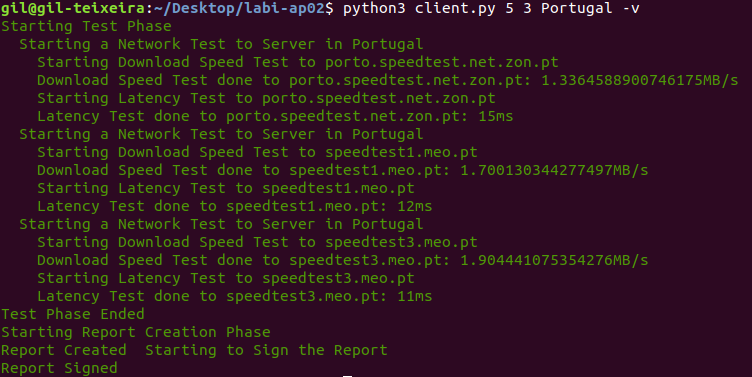
\includegraphics[width=\textwidth]{useExample}
Criando-se dois novos ficheiros na pasta onde está a aplicação:
\begin{itemize}
\item report.sig, contendo uma assinatura do relatório pela chave privada fornecida (\textit{key.priv}).
\item report.csv, um ficheiro \ac{csv} com os resultados dos três testes efetuados:
\end{itemize}
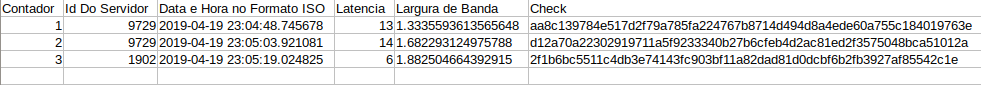
\includegraphics[width=\textwidth]{reportcsv}



\chapter*{Acrónimos}
\begin{acronym}
\acro{ua}[UA]{Universidade de Aveiro}
\acro{miect}[MIECT]{Mestrado Integrado em Engenharia de Computadores e Telemática}
\acro{guiaomini}[Mini-projeto]{Universidade de Aveiro
		Dep. de Electrónica, Telecomunicações e Informática
		Laboratório de Sistemas Digitais}
\acro{csv}[CSV]{Comma-separated values}
\end{acronym}
%%%%%%%%%%%%%%%%%%%%%%%%%%%%%%%%%



%%%%%%%%%%%%%%%%%%%%%%%%%%%%%%%%%


\end{document}
